\subsection{Motivation}
Modular synthesizers have seen continuous growth in popularity over the past decade, with the Eurorack format establishing itself as the dominant standard for modular synthesis hardware.
The ModularGrid database, a community-maintained catalogue of Eurorack modules, lists over 11,700 distinct modules from manufacturers ranging from large commercial companies to small community projects --- of which over 9,400 remain in active production today \cite{ModulesModularGrid}.
Despite the scale of this ecosystem, commercially available modules are often closed-source, expensive, and offer limited flexibility for experimentation with novel DSP algorithms.

Developing a custom DSP-capable Eurorack module from the ground up offers a unique opportunity to explore the full hardware-firmware stack --- from analog signal conditioning and PCB design to real-time audio processing on embedded hardware.
The STM32H7 platform, with its Cortex-M7 core running at up to 280\,MHz and hardware floating-point support, is a well-established target for embedded audio applications and provides sufficient computational headroom for the DSP workloads explored in this thesis.

\subsubsection{What is Eurorack?}
%TODO Image of patched Eurorack synth
%TODO Sources
Eurorack is a modular synthesizer format originally specified in 1995 by Dieter Doepfer with the introduction of the A-100 system --- the first modular synthesizer built around the format that now bears its name \cite{ZeittabelleDeutschEnglisch}.

\begin{wrapfigure}{r}{0.44\textwidth}
    \centering
    \vspace{-1em}
    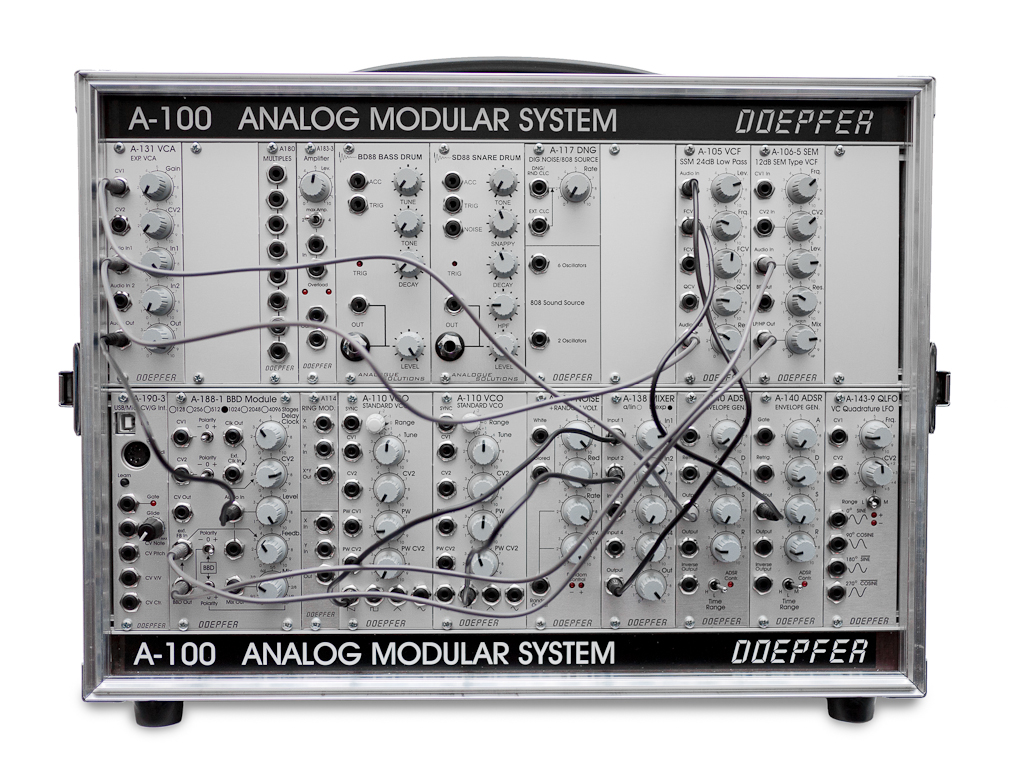
\includegraphics[width=0.4\textwidth]{../images/eurorack_fundamentals/Doepfer_A-100.jpg}
    \vspace{-0.9em}
    \caption{Doepfer A-100 System Variant}
    \vspace{-1.6em}
    \label{fig:a-100}
\end{wrapfigure}

The format defines mechanical, electrical, and signal standards that allow modules from different manufacturers to be combined freely in the same case, a property that has been central to its adoption.
In the mid to late-2000s, manufacturers such as Make Noise and TipTop Audio began producing compatible modules, and the ecosystem has grown continuously since \cite{SOSGuideChoosing}. 

The appeal of Eurorack lies in the big number of available modules: with so many modules to choose from, no two systems are alike.
Each module contributes its own sonic character and workflow, and together they form a highly individual electronic instrument.
However, the barrier to entry remains significant.

The high price point of Eurorack modules is a direct consequence of small production 
runs and significant development effort; a module from a boutique manufacturer may 
sell only a few hundred units, making economies of scale unavailable \cite{douglasAreModularSynths2023}.
This creates a natural motivation for open, community-driven hardware development 
as an alternative path into the ecosystem.


\subsection{Objectives}
The primary objective of this thesis is the development of a fully functional, DSP-capable Eurorack synthesizer module, encompassing the following:

\begin{itemize}
	\item Design and implementation of a Eurorack-compliant analog frontend, including CV input conditioning, V/Oct pitch tracking, and audio codec interfacing
	\item Development of a real-time firmware architecture on the STM32H7 platform using FreeRTOS, meeting the latency and stability requirements of a live performance instrument
	\item Implementation of a tape-loop playback engine with pitch shifting, supporting real-time CV control
	\item Investigation of pitch interpolation algorithms suitable for embedded real-time audio
	\item Implementation and evaluation of a Schroeder reverb algorithm as a secondary DSP focus point
	\item Verification of the complete system against defined hardware and firmware requirements
\end{itemize}